\chapter{文獻回顧}




\cite{radiometry_and_photometry}


本研究所探討情境下的量測方法有以下需求:有易於拆裝的量測單位與被量測單位,能夠快速進行拆裝、靈活應用於不同場域,而安裝完成後即可進行三維相對位置量測。為滿足靈活且易於安裝且能夠應用在不同場域的特性,需要有體積小、能耗低、所需校正步驟少、能夠使用於不同場域等特色。

因此,本章節先定義所謂相對定位,再介紹現有文獻的定位技術與方法,比較優缺點並凸顯「近紅外光定位」的優勢,近而針對本論文著重的「LED與PD以近紅外光波段進行定位」的文獻進行探討,敘述此領域研究現況與困難。







% 重申自己主要的目標:(只有LED-PD近紅外光波段符合的原因)
% 低成本、不需預先了解環境資訊、裝設範圍小、方便架設、速度

\section{相對定位定義}
% -(利用數學符號描述相對定位問題的定義(軌跡、時間等))
    
    在開始進入文獻探討之前,需先以數學定義何謂本論文所欲量測之「相對定位」。首先,本論文所討論的情境為一量測物針對另一特定目標物進行相對位置的量測,如智慧工廠內的機械手臂欲取得與移動載具之間的相對關係,以利夾取搬運物品至載具上進行運送。
    
    我們將取得相對位置的一方稱為量測者,如案例中的機械手臂;而量測者所欲取得相對位置的特定物體稱為目標物,如案例中的移動載具;兩者皆為剛體。因此,可以將量測者與目標物各自視為兩移動座標系如圖\ref{pic:homo_trans},兩者在空間中各自有位置、旋轉的六個自由度,可以利用齊次座標轉換(Homogeneous Transformation)表示座標系之間的平移與旋轉(式\ref{eqn:homogeneous}),$^{PL}\boldsymbol{H}$表示將LED座標系上的點轉換至PD座標系上的齊次轉換矩陣,而$^{PL}\boldsymbol{T}$與$^{PL}\boldsymbol{Ro}$各自代表平移與旋轉的轉換矩陣,符號可參考符號列表(第\pageref{chp:symbol}頁)。
  
    \begin{equation}
    \label{eqn:homogeneous}
    \begin{gathered}
        \left[
        \begin{array}{c}
            ^{PL}P \\1
        \end{array}\right]
        =^{PL}\boldsymbol{H}
        \left[
        \begin{array}{c}
        ^{L}P \\ 1
        \end{array}\right] =\left[
        \begin{array}{cc}
        ^{PL}\boldsymbol{Ro} & ^{PL}\boldsymbol{T} \\
        0 & 1
        \end{array}\right]\left[
        \begin{array}{c}
        ^{L}P \\ 1
        \end{array}\right] \\
    \end{gathered}
    \end{equation}

    \begin{equation}
        ^{PL}\boldsymbol{T}=\left[\begin{array}{l}
        ^{PL}x \\ ^{PL}y \\ ^{PL}z
        \end{array}\right]
    \end{equation}

    \begin{figure}[ht]
        \centering
        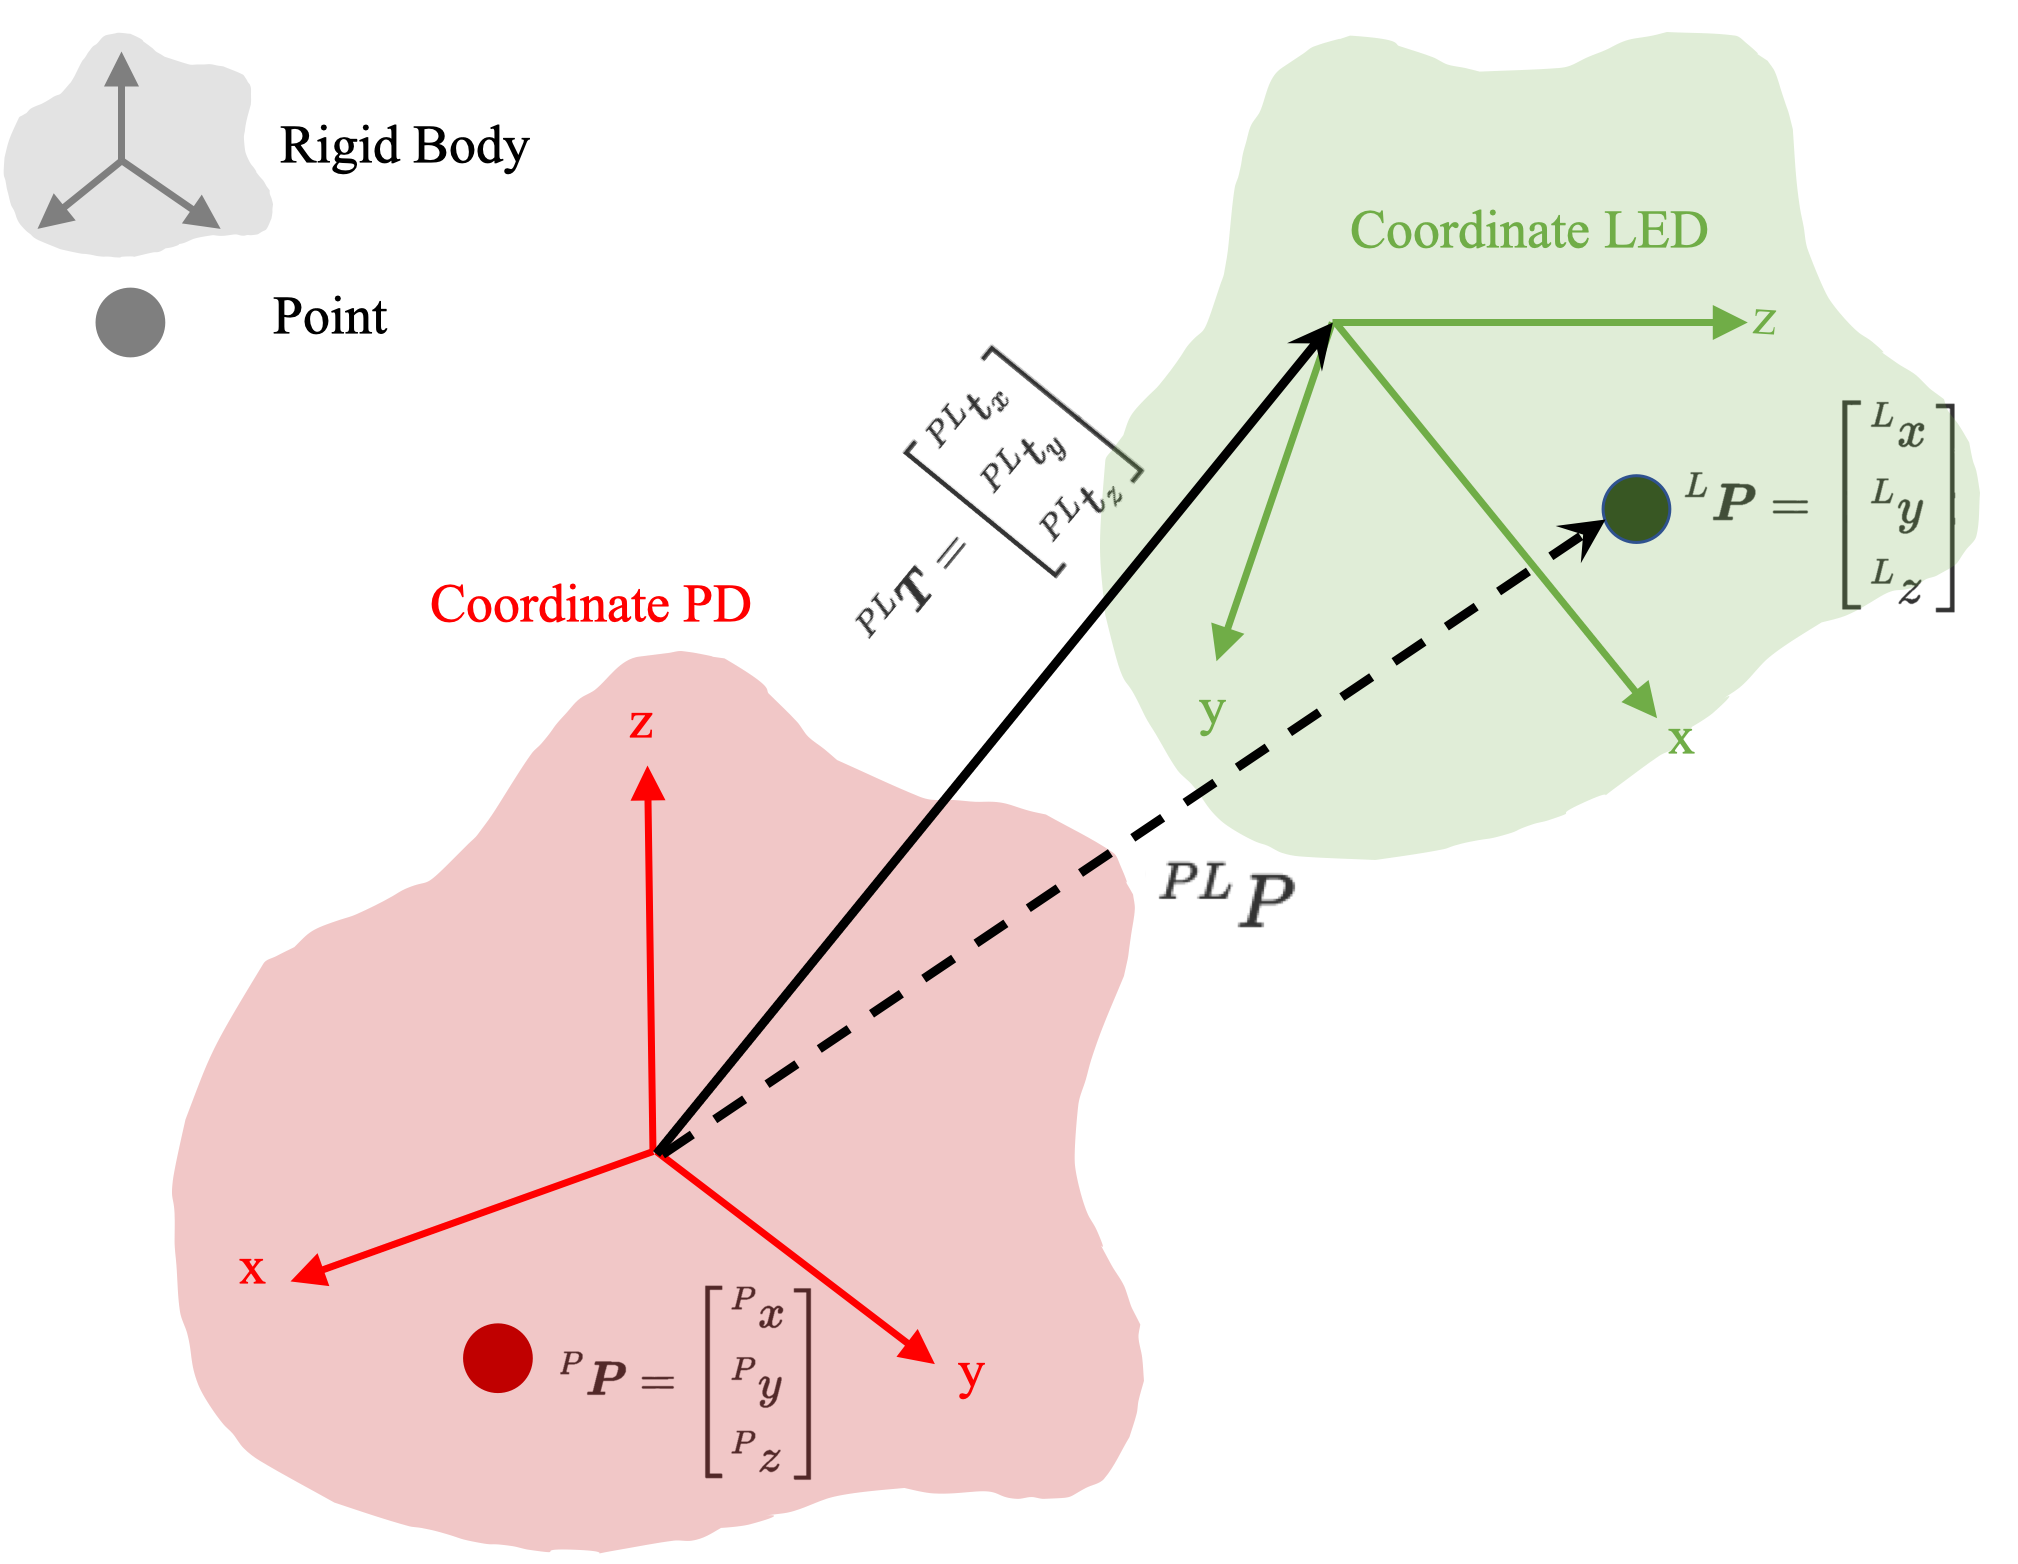
\includegraphics[width=9cm]{ch2pic/homo_trans.png}
        \caption{LED座標系與PD座標系及相對關係}
        \label{pic:homo_trans}
    \end{figure}
    
   其中,兩座標系之間的平移關係$^{PL}\boldsymbol{T}$即為欲得到的相對位置資訊,共有三個自由度。

 



\section{定位方法介紹}
(這段或許可以省略)
    - 定位方法介紹:RSS、TDOA這些
    
    % (Ref幾篇Review)
    
    - 先用方法得到角度、距離資訊:利用RSS、TDOA比較
    - 組合角度、距離資訊得到位置:Multitrileration, Fingerprinting

\section{定位技術介紹}

    定位所使用的技術十分多樣,包含使用電磁波段內的Wifi、藍芽、RFID、可見光、以及相機定位等,以及其他定位技術如超聲波等。

    \subsection{以電磁波頻率切入}

        電磁波段內也有許多不同的量測手段,包含了可見光定位、視覺辨識、光達、藍芽、RFID等現今受到關注的量測方法,其中電磁波以光速傳播,傳遞速度為一優勢,再來不需傳遞介質的特性使其傳遞速度不受環境溫度、濕度影響,減少可能對量測訊號造成影響的變因。

        電磁波段內本段落為分類不同量測方法,從電磁波的頻率波長特性切入。電磁波頻率越高所含能量越高,此特性使得高頻波段(X光波段等)對人體有害,因此無法使用於定位。同樣在光波段內,紅外光因能量較小、於視網膜成像的難故也大,因此較可見光安全。
        
        電磁波段另一個特性為波長愈短可達到的定位經度愈高,且量測與發射的硬體單位大小愈小,市售常見的光波段感測器如感光二極體(Photodiode)尺寸
        
        綜上所述,根據本研究目標所需,將研究方法聚焦在光波段的定位上。

    \subsection{光波段定位}

        光波段的定位發展近幾年來十分顯著,主要原因為光學硬體上的進步,以及可見光通訊的發展。

        光波段的分類可從兩方向切入:使用波段與感測器硬體選擇。

        比較可見光與紅外光:(研究普及度、誤差、對眼睛干擾)

        研究普及度:

        首先,現今室內定位的研究主要著重在可見光的部分,搭配著室內環境都具有的光源,在不對室內環境進行過多改動上即可進行定位量測。然而本研究需能靈活將光源安裝於任意被觀察物上,因此室內充足的可見光光源並不能成為訊號載體,因此在挑選光波段的部分著重在降低誤差上。

        硬體價格:

        普遍對紅外光波段的硬體都有價格昂貴的印象,此原因是在超過??波段的感光與發光硬體,並不能單純使用矽,特殊的硬體加工方式使紅外光波段的硬體價格昂貴,然而可見光與近紅外光波段並不受此限。

        誤差:

        光波段的誤差來源主要包含Ambious Light Source, Multipath effect等,其中環境光強度過高可造成訊號偏移甚至硬體飽和導致訊號失真,因此需有效的降低環境光源的強度以保持定位的準確度。環境光源包含了室內的光源以及太陽光源,室內的光源的頻率約在120hz??,可以針對頻率進行濾波,而太陽光源的強度則隨頻率增減。從太陽光頻譜圖可以觀察到,太陽光於光波段受到大氣層吸收有三處的能量較低,藉由挑選低谷頻率,即可有效降低太陽光對系統的影響。

        對眼睛的影響:

        紅外光在本研究上有另一優勢,其裝載在一動物體上,即使光源在環境中的使用者面前不停閃爍、直射,紅外光無法在視網膜成像的特性讓使用者並不會受到影響,反之,朝人眼照射的可見光源會干擾。

        [可做一張十字圖:(相機vsPD)(可見光vs紅外光)]

        [Ref頻譜圖,強調選用波段]

        權衡之下,挑選於太陽光輻射光譜中低谷的??hz波段,同時享有硬體多且價格低的優勢,又減少了太陽光源所影響的程度,使裝置保持輕巧低成本又不干擾人眼與日常生活的優點。

\section{LED與PD的定位方法}

    LED與PD的定位方式,是將單個或多個LED安裝在目標物上,各LED藉由編碼來區別各自的訊號,而PD安裝於觀察物上,將每個PD所接收的訊號分別解碼,得到各LED的訊號強度。

    為深入了解系統運作方式,從基本的光領域常用單位切入,開始介紹LED與PD的硬體特性與參數,以及光傳播上的模擬建模,再進入系統整體的細節。

    \subsection{光領域基本介紹}
        由於光領域所使用的單位與機械領域差距較大,進入PD與LED定位的探討之前,先對光領域的一些術語與單位進行介紹。

        在描述光波的單位在文獻上經常有些混亂,單位分為兩種制度常令人感到困惑;而不同文獻口語稱呼單位的方式皆不同,例如「強度」在不同文獻可代表通量、輻射強度、輻照度等不同單位,因此以下進行釐清。
        
        首先,光領域中的計量單位大致分成兩種系統:輻射測量學(Radiometry)與光度測量學(Photometry),兩領域以不同單位描述光源,其中輻射測量學著重在電磁波輻射的量測,描述通量單位為瓦特(Watt);而光度測量學著重在人演可見之可見光波段的研究,通量單位為流明(Lumen),單位定義不同。
        
        本論文中著重在紅外光波段,因此使用的單位系統為輻社測量學的系統,然而文獻上可見光定位數量較多,因此在單位的換算上需特別注意。
        
        再來,無論中文英文的文獻,常見文獻或口語上使用同一詞但指不同物理量,在描述物理量上需避免重複或是混亂,閱讀上最好確認「單位」是否正確。本文所使用之單位系統為輻社測量學,物理量與單位對照如表格所示。

        光源存在於立體空間中,描述二維空間中的角度單位為弧度,而空間中描述角度的物理量為立體角(Solid Angle),單位為球面度(steradians, 簡寫sr)。其定義如下:r單位半徑長的球體中,立體角

        描述光照總能量的物理量單位為通量(Flux)或稱輻射功率,代表每單位時間的輻射能量,每單位立體角所含的通量稱為輻射強度、每單位面積所含的通量稱為輻照

    \subsection{LED與PD的硬體參數與特性}

        為建立一完整描述光傳遞的模型,需先介紹實際實際硬體挑選時所需注意的參數。

        首先LED包含總輻射強度、半角度
        
        LED與PD硬體有許多種類,最常見的市面上LED與PD為軸對稱並滿足Lambertian Radiation Pattern,本論文也只考慮此類硬體。軸對稱代表當LED或PD僅對出射角或入射角以及距離有敏感度,以球座標系來看,凡在同一仰角與距離,無論方位角為何,光照強度與感光強度皆相同。

    \subsection{光傳遞模型}

        LED與PD的照射與接收模式(Pattern)可以用Lambertian Radiation Pattern量化,代表感光與發光強度隨著LED出射角與PD入射角的增加而變小,其衰減模式可用餘弦函數(cosine)的M次方(power)表示,M代表的是Lambertian Order。

        以二維的角度來看如圖,LED光照射的能量隨出射角度增加而減少,在LED中心軸的方向強度最高,在此描述LED強度時不考慮距離。如先前所述,LED為軸對稱,因此三維的照射模式即為二維模式以中心軸旋轉。在同樣出射角下,光intensity相同。
        
        有了光intensity在不同入射角的關係,將整個半球中的intensity積分,得到LED在整個半球上所照射的總瓦數比例,將該值倒數,即可由LED發射之總能量推算各入射角的光intensity。
        
        討論完LED與角度的關係後,再來考慮光能量與距離的關係。考慮同一Solid angle下的一束光,隨傳遞距離拉長,所照射到的表面積增加,因此「能量」隨距離平方遞減。
        
        綜合角度與距離的影響,空間中任一點的「光大小」如式
        
        接著考慮PD接收的Model,PD的接收能量與入射角同樣遵守Lambertian Pattern,變數一樣包含入射角以及Lambertian Order。除了角度以外,藉由乘上PD的硬體參數感光面積得到該PD所感測到的瓦數,PD會將感受到的光瓦數轉換為電流輸出,其中轉換比例為Responsivity。
        
        舉具體的例子來描述lambertian order的影響,M越大的LED,光強度隨出射角度衰減的速度越大,而照射範圍則越小。在挑選硬體時,M的選擇則為強度與範圍的取捨。同樣總輻射能量的LED,不同M隨角度的發光強度如圖示,首先可以觀察到M越小所覆蓋的角度範圍越大,而中心軸的光強度也小很多,其原因是因為其照射範圍大,因此在半球面上大角度的積分,入射角度越大時在半球面上的面積越大。
        
        從硬體層面來看,LED與PD的照射範圍

    \subsection{LED與PD定位系統}

        以LED與PD量測系統為例,目標物為LED座標系,剛體上裝載著主動發送訊號的LED;而量測者為PD座標系,上面裝載著傳感器收取資訊;兩座標系上的感測器與訊號發送器皆為固定的,可以想像成將PD焊於電路板上,封裝成一量測儀器,並以螺絲等固定在量測者剛體上,隨著量測者與目標物移動時,兩座標系之間的座標轉換關係會改變,然而PD與其座標轉換關係並不會改變,LED亦然。

    \subsection{LED與PD定位文獻探討}

        了解LED與PD定位系統的運作方式後,本章節介紹現有文獻的成果,並舉實例情境來凸顯此領域不足之處,提出可改善之方向。

\section{結論}

雖然此種做法已被討論且有潛力,但缺少完整考慮[組態、硬體參數]的方式,因此本論文補上